% ********** Rozdział 2 **********
\chapter{Opis struktury projektu}

\section{Opis Struktury Projektu}
System zarządzania dokumentami został zaprojektowany w języku \textbf{C\#}, wykorzystując programowanie obiektowe (OOP). Struktura projektu składa się z kilku głównych klas, które odpowiadają za przechowywanie, zarządzanie i przetwarzanie dokumentów.


\subsection{Diagram Klas}
Poniżej przedstawiono diagram klas ilustrujący hierarchię obiektów w systemie:

\begin{center}
    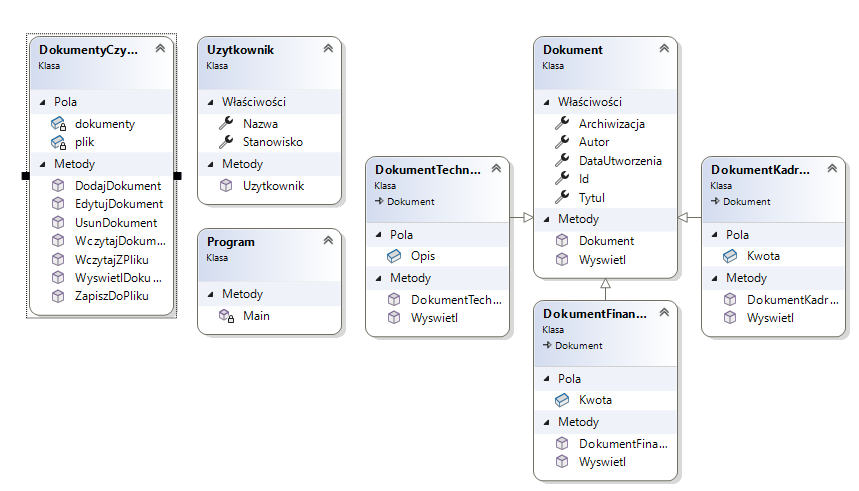
\includegraphics[width=0.8\textwidth]{diagramklas.png}
\end{center}


\subsection{Klasa bazowa: Dokument}
\begin{itemize}
\item Właściwości: \texttt{Id}, \texttt{Tytul}, \texttt{Autor}, \texttt{DataUtworzenia}, \texttt{CzyZarchiwizowany}
\item Metoda abstrakcyjna: \texttt{WyswietlInformacje()}
\end{itemize}

\subsection{Klasy pochodne:}
\begin{itemize}
\item \textbf{DokumentFinansowy} (\texttt{Kwota} jako dodatkowa właściwość)
\item \textbf{DokumentKadrowy} (\texttt{Pracownik} jako dodatkowa właściwość)
\item \textbf{DokumentTechniczny} (\texttt{Opis} jako dodatkowa właściwość)
\end{itemize}

\subsection{Klasa Użytkownik}
\begin{itemize}
\item Właściwości: \texttt{Nazwa}, \texttt{Rola}
\item Reprezentuje użytkowników z różnymi uprawnieniami (Administrator, Pracownik, Gość)
\end{itemize}

\subsection{Klasa DokumentyCzynnosci}
\begin{itemize}
\item Metody:
\begin{itemize}
\item {DodajDokument}\texttt{(Dokument dokument, Użytkownik użytkownik)}
\item {UsunDokument}\texttt{(int id, Użytkownik użytkownik)}
\item {EdytujDokument}\texttt{(int id, string nowyTytul, string nowyAutor, bool nowaArchiwizacja, Użytkownik użytkownik)}
\item {WczytajZPliku()}
\item {ZapiszDoPliku()}
\item {WyswietlDokumenty()}
\end{itemize}
\end{itemize}

\subsection{Klasa Program (obsługa interfejsu użytkownika)}
\begin{itemize}
\item Menu umożliwiające wybór operacji na dokumentach
\item Wczytywanie danych przy starcie aplikacji
\item Obsługa logowania użytkownika
\end{itemize}

\section{Opis Techniczny}
\subsection{Język Programowania i Narzędzia}
Projekt został napisany w języku \textbf{C\#} w środowisku \textbf{Microsoft Visual Studio 2022}. 

\subsection{Minimalne Wymagania Sprzętowe}
\begin{itemize}
    \item Procesor: Intel Core i3 lub wyższy
    \item Pamięć RAM: 4 GB
    \item System operacyjny: Windows 10/11
    \item Dysk: Minimum 200 MB wolnej przestrzeni
\end{itemize}

\section{Zarządzanie Danymi i Baza Danych}
Dane są przechowywane w pliku tekstowym \texttt{dokumenty.txt}. Każdy dokument jest zapisywany w postaci linii danych oddzielonych separatorem \texttt{|}






% ********** Koniec rozdziału **********
